% Generated by src/eda.py. Needs \usepackage{graphicx}.
% Upload figures/eda_combined.pdf to your Overleaf project's figures/ folder.
% figure* spans both columns in the two-column IEEE layout.
\begin{figure*}[t]
  \centering
  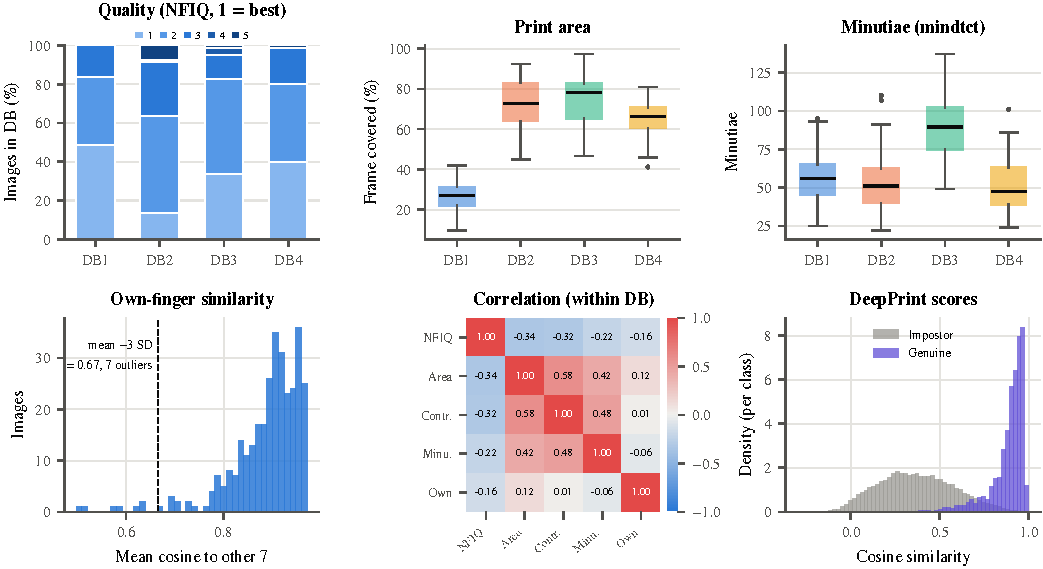
\includegraphics[width=\textwidth]{figures/eda_combined.pdf}
  \caption{\textbf{Exploratory data analysis of FVC2004 Set~B.} Top row, univariate image quality by sensor: NFIQ, print area, and minutiae count. Bottom row, the own-finger similarity distribution with its 3-SD outlier cut, the within-DB correlation of image statistics (Spearman), and the genuine/impostor DeepPrint score distributions. The four sensors differ sharply in quality, no single statistic predicts matching difficulty within a sensor ($|\rho|\le0.16$), and the impostor and genuine classes overlap only in the tail.}
  \label{fig:eda-combined}
\end{figure*}
